\documentclass{article}

\usepackage{circuitikz}
\usetikzlibrary{external}

\begin{document}

\begin{tikzpicture}[> = latex]

	% Definitions
	
	\def\a{3} 		% (Semi-)major axis
	\def\b{2.5} 		% (Semi-)minor axis
	\def\Q{220}		% Mass position along orbit
	\def\L{1}		% Size of angle indicator in vector diagram
	
	% Calculate linear eccentricity
	
	\pgfmathparse{sqrt(\a^2 - \b^2)}
	\let\c\pgfmathresult
	
	\coordinate (M-pos) at (\c, 0);
	
	% Velocity component along radial vector
	
	\pgfmathparse{((\a^2 - \b^2) * sin(\Q) * cos(\Q) - \a * \c * sin(\Q))/ ((\c - \a * cos(\Q))^2 + \b^2 * sin(\Q)^2)}
	\let\vPar\pgfmathresult
	
	% Velocity component perpendicular to radial vector
	
	\pgfmathparse{(\b * \c * cos(\Q) - \a * \b)/ ((\c - \a * cos(\Q))^2 + \b^2 * sin(\Q)^2)}
	\let\vPerp\pgfmathresult
	
	% Unit vector along radial vector
	
	\pgfmathparse{1 / ((\c - \a * cos(\Q))^2 + \b^2 * sin(\Q)^2)}
	\let\unitPar\pgfmathresult
	
	% Unit vector along perpendicular vector
	
	\pgfmathparse{1 / ((\c - \a * cos(\Q))^2 + \b^2 * sin(\Q)^2)}
	\let\unitPerp\pgfmathresult

	% Elliptical orbit
	
	\draw [dashed] (0, 0) circle [x radius = \a, y radius = \b];
	
	% Mass along orbit + radial line
	
	\draw [dotted] (M-pos) -- ({\a * cos(\Q)}, {\b * sin(\Q)});
	
	\draw [ball color = red!50] ({\a * cos(\Q)}, {\b * sin(\Q)}) circle (4 pt) coordinate (m-pos);
	\node [left = 0.5 em] at (m-pos) {$P$};
	
	% Place the large mass M at the right-hand focus; use the
	% linear eccentricity for the x coordinate
	
	\draw [ball color = yellow] (M-pos) circle (4 pt);
	\node [above = 0.5 em] at (M-pos) {$S$};
	
	% Velocity vector diagram at mass position
	
	\draw [->] ({\a * cos(\Q)}, {\b * sin(\Q)}) -- node [midway, above] {$v_r$} ++ ({\vPar * (\c - \a * cos(\Q))}, {-\vPar * \b * sin(\Q)}) coordinate (end-vr);
	\draw [->] (end-vr) -- node [midway, above right] {$v_\perp$} ++ ({\vPerp * \b * sin(\Q)}, {\vPerp * (\c - \a * cos(\Q))});
	\draw [very thick, ->] ({\a * cos(\Q)}, {\b * sin(\Q)}) -- node [midway, below left] {${\vec v}$} ++ ({-\a * sin(\Q)}, {\b * cos(\Q)});
	
	% Angle indicator in vector diagram
	
	\draw [thin, gray] (end-vr) ++ ({-\L * \unitPar * (\c - \a * cos(\Q))}, {\L * \unitPar * \b * sin(\Q)})
		-- ++ ({-\L * \unitPerp * \b * sin(\Q)}, {-\L * \unitPerp * (\c - \a * cos(\Q))})
		-- ++ ({\L * \unitPar * (\c - \a * cos(\Q))}, {-\L * \unitPar * \b * sin(\Q)});
	
\end{tikzpicture}

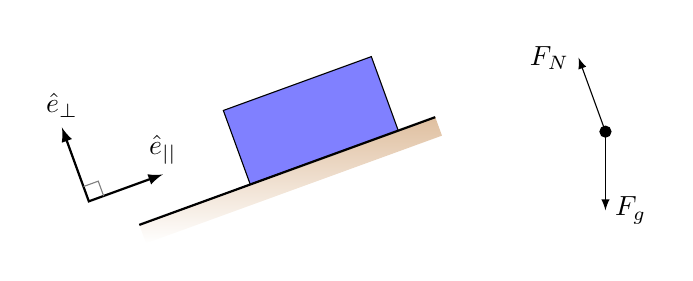
\begin{tikzpicture}[> = latex]

	% Definitions
	
	\def\Q{20}		% Ramp angle
	
	\matrix[column sep = 1 cm, ampersand replacement = \&]{
	
	% Actual picture, rotated

	\begin{scope}[rotate = \Q]
		
		% Block
		
		\draw [fill = blue!50] (-0.5, 0) rectangle (1.5, 1);
	
		% Ramp surface
	
		\draw [draw = none, top color = brown!50, bottom color = white] (-2, 0) rectangle (2, -0.25);
		\draw [thick] (-2, 0) -- (2, 0);
		
		% Unit vectors + perpendicular angle indicator
		
		\draw [<->, thick] (-2.5, 1.5) node [above] {${\hat e}_\perp$} -- (-2.5, 0.5) -- (-1.5, 0.5) node [above] {${\hat e}_{||}$};
		\draw [thin, gray] (-2.3, 0.5) -- (-2.3, 0.7) -- (-2.5, 0.7);
	
	\end{scope}
	
	\&
	
	% FBD
	
	\begin{scope}[yshift = 0.5 cm]
	
		\draw [fill = black] (0, 0) circle (2 pt);
		
		\draw [->] (0, 0) -- (0, -1) node [right] {$F_g$};
		\draw [->] (0, 0) -- (90 + \Q : 1) node [left] {$F_N$};
	
	\end{scope}
	
	\\
	};

\end{tikzpicture}

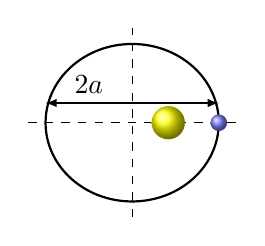
\begin{tikzpicture}[> = latex]

	% Definitions
	
	\def\semiMajor{1.1}	% Horizontal distance for ellipse
	\def\semiMinor{1}		% Vertical distance for ellipse
	\def\R{3}
	
	% Axes
	
	\draw [dashed] (-1.2 * \semiMajor, 0) -- (1.2 * \semiMajor, 0);
	\draw [dashed] (0, -1.2 * \semiMinor) -- (0, 1.2 * \semiMinor);
	
	% Lable semi-major axis
	
	\draw [<->] (-\semiMajor, 0.25) -- node [near start, above] {$2a$} (\semiMajor, 0.25);
	
	% Elliptical orbit
	
	\draw [thick] (0, 0) ellipse [x radius = \semiMajor, y radius = \semiMinor];
	
	% Sun at right focus
	
	\shade [ball color = yellow] ({sqrt(\semiMajor * \semiMajor - \semiMinor * \semiMinor)}, 0) circle (2 * \R pt);
	
	% Planet
	
	\shade [ball color = blue!50] (\semiMajor, 0) circle (\R pt);

\end{tikzpicture}

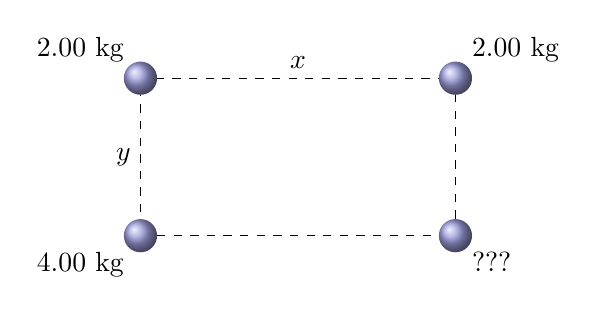
\begin{tikzpicture}

	% Dashed lines for distances
	
	\draw [dashed] (0, 0) -- (4, 0) -- (4, 2) -- node [midway, above] {$x$} (0, 2) -- node [midway, left] {$y$} (0, 0);
	
	% Masses at corners
	
	\begin{scope}[ball color = blue!50!gray!50]
	
		\shade (0, 0) circle (6 pt) node [below left = 0.25 em] {4.00 kg};
		\shade (0, 2) circle (6 pt) node [above left = 0.25 em] {2.00 kg};
		\shade (4, 0) circle (6 pt) node [below right = 0.25 em] {???};
		\shade (4, 2) circle (6 pt) node [above right = 0.25 em] {2.00 kg};
	
	\end{scope}

\end{tikzpicture}

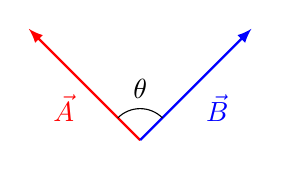
\begin{tikzpicture}[> = latex]

	\begin{scope}[->, thick]
	
		\draw [red] (0, 0) -- node [below left] {${\vec A}$} (135 : 2);
		\draw [blue] (0, 0) -- node [below right] {${\vec B}$} (45 : 2);
	
	\end{scope}

	\draw (135 : 0.4) arc (135 : 45 : 0.4);
	\node at (90 : 0.65) {$\theta$};

\end{tikzpicture}

\begin{tikzpicture}[> = latex]
\matrix[column sep = 1 cm]{

	\begin{scope}[->, thick]
	
		\draw [red] (0, 0) -- node [below right] {${\vec A}$} (225 : 2);
		\draw [blue] (0, 0) -- node [above] {${\vec B}$} (0 : 2);
	
	\end{scope}
	
	\node at (0, -2) {A.};
	
	&

	\begin{scope}[->, thick, yshift = -1.2 cm]
	
		\draw [red] (0, 0) -- node [below right] {${\vec A}$} (30 : 2);
		\draw [blue] (0, 0) -- node [below left] {${\vec B}$} (120 : 2);
	
	\end{scope}
	
	\node at (0, -2) {B.};
	
	&

	\begin{scope}[->, thick, yshift = -0.5 cm]
	
		\draw [red] (0, 0) -- node [above] {${\vec A}$} (2, 0);
		\draw [blue] (2, 0) -- node [above] {${\vec B}$} (4, 0);
	
	\end{scope}
	
	\node at (2, -2) {C.};
	
	&

	\begin{scope}[->, thick, yshift = 0.5 cm]
	
		\draw [red] (0, 0) -- node [above left] {${\vec A}$} (260 : 2);
		\draw [blue] (0, 0) -- node [above right] {${\vec B}$} (280 : 2);
	
	\end{scope}
	
	\node at (0, -2) {D.};

\\
};

\end{tikzpicture}

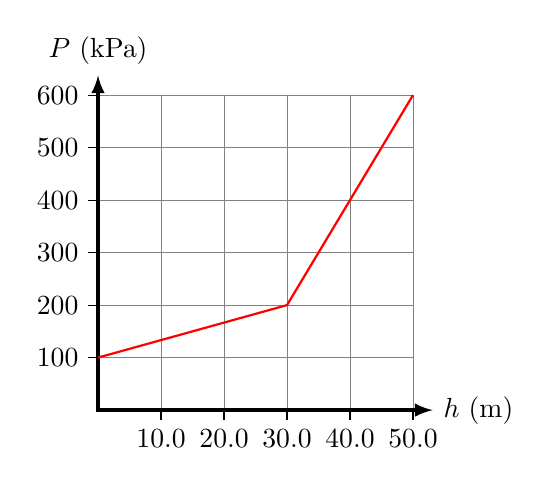
\begin{tikzpicture}[> = latex]

	% Graph grid + axes
	
	\draw [very thin, gray, xstep = 0.8, ystep = {2/3}] (0, 0) grid (4, 4);
	\draw [very thick, <->] (0, 4.25) node [above] {$P$ (kPa)} -- (0, 0) -- (4.25, 0) node [right] {$h$ (m)};
	
	% Graph labels
	
	\foreach \P in {100, 200, ..., 600}
		\draw (0, \P/150) -- (-0.125, \P/150) node [left] {\P};
	
	\foreach \h in {10.0, 20.0, 30.0, 40.0, 50.0}
		\draw (0.08 * \h, 0) -- (0.08 * \h, -0.125) node [below] {\h};
		
	% Graph curve
	
	\draw [red, thick] (0, 2/3) -- (2.4, 4/3) -- (4, 4);
	
\end{tikzpicture}

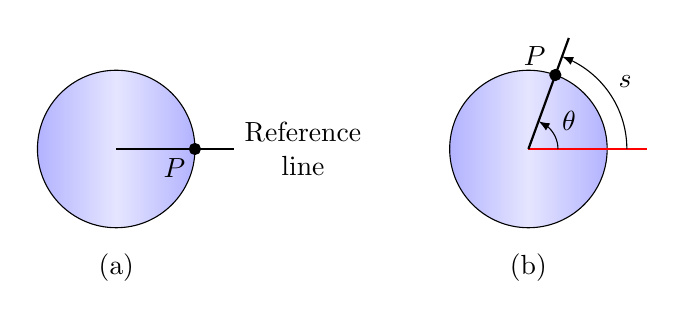
\begin{tikzpicture}[> = latex]
\matrix[column sep = 1 cm]{

	\draw [left color = blue!30, right color = blue!30, middle color = blue!10] (0, 0) circle (1 cm);
	
	\draw [thick] (0, 0) -- (1.5, 0) node [right, align = center] {Reference\\line};
	
	\draw [fill = black] (1, 0) circle (2 pt) node [below left] {$P$};
	
	\node at (0, -1.5) {(a)};
	
&

	\draw [left color = blue!30, right color = blue!30, middle color = blue!10] (0, 0) circle (1 cm);
	
	\draw [red] (0, 0) -- (1.5, 0);
	\draw [thick] (0, 0) -- (70 : 1.5);
	
	\draw [->] (0.375, 0) arc (0 : 70 : 0.375) node [right = 0.5 em] {$\theta$};
	\draw [->] (1.25, 0) arc (0 : 70 : 1.25);
	\node at (35 : 1.5) {$s$};
	
	\draw [fill = black] (70 : 1) circle (2 pt) node [above left] {$P$};
	
	\node at (0, -1.5) {(b)};
	
\\
};

\end{tikzpicture}

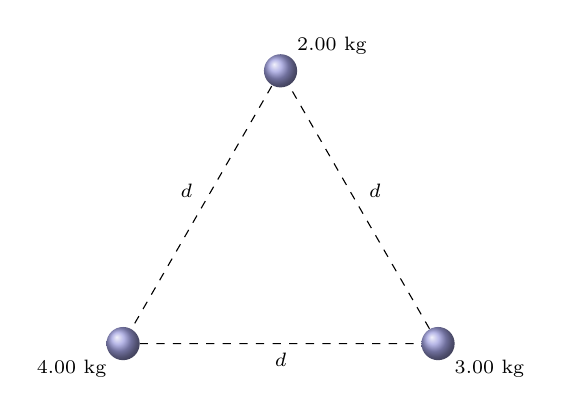
\begin{tikzpicture}[every node/.style = {font = \scriptsize}]

	% Dashed lines for distances
	
	\draw [dashed] (-2, 0) -- node [midway, below] {$d$} (2, 0) -- node [midway, above right] {$d$} (0, {sqrt(12)})
		-- node [midway, above left] {$d$} (-2, 0);
	
	% Masses at corners
	
	\begin{scope}[ball color = blue!50!gray!50]
	
		\shade (-2, 0) circle (6 pt) node [below left = 0.25 em] {4.00 kg};
		\shade (2, 0) circle (6 pt) node [below right = 0.25 em] {3.00 kg};
		\shade (0, {sqrt(12)}) circle (6 pt) node [above right = 0.25 em] {2.00 kg};
	
	\end{scope}
	
\end{tikzpicture}

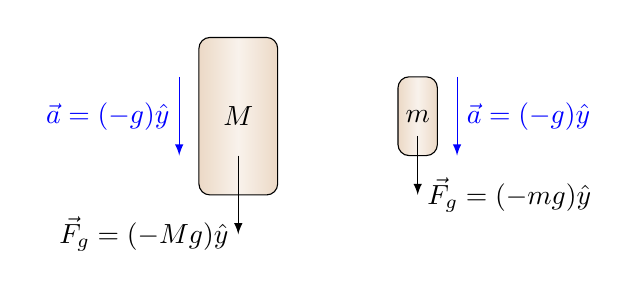
\begin{tikzpicture}[> = latex]
\matrix[column sep = 1.5 cm]{
	
	\draw [left color = brown!30, right color = brown!30, middle color = brown!10, rounded corners] (-0.5, -1) rectangle (0.5, 1);
	\node at (0, 0) {$M$};
	
	\draw [->] (0, -0.5) -- (0, -1.5) node [left] {${\vec F}_g = (-Mg) {\hat y}$};
	
	\draw [->, blue] (-0.75, 0.5) -- node [left] {${\vec a} = (-g) {\hat y}$} (-0.75, -0.5);
	
&
	
	\draw [left color = brown!30, right color = brown!30, middle color = brown!10, rounded corners] (-0.25, -0.5) rectangle (0.25, 0.5);
	\node at (0, 0) {$m$};
	
	\draw [->] (0, -0.25) -- (0, -1) node [right] {${\vec F}_g = (-mg) {\hat y}$};
	
	\draw [->, blue] (0.5, 0.5) -- node [right] {${\vec a} = (-g) {\hat y}$} (0.5, -0.5);
	
\\
};
\end{tikzpicture}

\end{document}